\documentclass[11pt]{article}

%\pagestyle{empty}

\hyphenation{con-si-de-ra-to}

%\textwidth=182mm
%\textheight=230mm
%\hoffset=-31mm                  % horizontal offset
%\voffset=-30mm                  % vertical offset

\usepackage[margin=.775in]{geometry}

\usepackage[usenames]{color}
%\usepackage[mathcal]{eucal}
\usepackage{epsfig}
\usepackage{amsmath}
\usepackage{amssymb}
\usepackage{amsthm}
\usepackage{amsfonts}
\usepackage{enumerate}
\usepackage{amsthm}
\usepackage{dsfont}
\usepackage[usenames]{color}
\usepackage{wrapfig}
\usepackage{graphicx}
\usepackage{blindtext}
\usepackage{enumerate}
\usepackage{fancyvrb}
\usepackage{esint}

\usepackage{lscape}

\usepackage{color,hyperref}
\definecolor{darkblue}{rgb}{0.0,0.0,.45}
\definecolor{darkred}{rgb}{0.7,0,0}
\hypersetup{colorlinks,breaklinks,
	linkcolor=darkred,urlcolor=darkred,
	anchorcolor=darkred}


\newcommand{\myparallel}{{\mkern3mu\vphantom{\perp}\vrule depth 0pt\mkern2mu\vrule depth 0pt\mkern3mu}}

\newcommand{\qq}{\mathbf{q}}
\newcommand{\qqd}{\mathbf{\dot{q}}}
\newcommand{\ind}{\mathds{1}} % so $\ind{1}$ gives you the script 1
\newcommand{\gul}[2]{g^{#1 ,}_{\textcolor{White}{#1}#2\ }}

\theoremstyle{plain}
\newtheorem{corollary}{Corollary}
\newtheorem{proposition}{Proposition}
\newtheorem{lemma}{Lemma}
\theoremstyle{definition}
\newtheorem{definition}{Definition}
\newtheorem{example}{Example}
\newtheorem{case}{Case}
\newtheorem{conj}{Conjecture}
\newtheorem*{remark}{Remark}
\newtheorem*{notation}{Notation}
%\newtheorem{fc1}{From Chapter 1 of Millman \& Parker:}
%\newtheorem{fc2}{From Chapter 1 of Millman \& Parker:}
\newtheorem{problem}{Problem}
\newtheorem{theorem}{Theorem}
%\renewcommand*{\theproblem}{\hwn\Alph{problem}}
\renewcommand*{\theproblem}{\hwn.\arabic{problem}}
%\newtheorem{theorem}{Theorem}
\theoremstyle{remark}

\parindent=0cm

\newcommand{\hwn}{2}

\begin{document}
\LARGE
\noindent{\textsf{\textbf{CGU Math 381 (Image Processing), Spring '18 
			-- Homework \#\hwn}}}
\par\vspace{.25cm}
\Large
\hspace{.5cm}\textsf{\mbox{%
Edge detection, 
sharpening, the Total Variation norm, and histogram equalization. 
}}
\par\vspace{.2cm}
\normalsize
\hspace{.5cm}\mbox{\textsf{\em Due 
		on Tuesday 3/6, at the beginning of class. }%
}
\par\vspace{.3cm}
\normalsize\rm
%$\boxed{\mbox{ \bf This homework assignment is on two
%		 pages. }}$ \par\vspace{.3cm}
\bf Reading: \rm
While the class notes should be sufficient 
for this homework assignment, it is still useful to read 
Chapters~1 to~6 of \em Principles of Digital Image
Processing \em by Burger \& Burge. You may skip
all the parts that refer to Java implementations
and ImageJ (for example, all of Chapter~2).
\par\vspace{.15cm}
Write, on top of the first page of your assignment:
Name (\underline{LAST}, First), your University or College, the HW\#, and acknowledge other students
with whom you may have worked (just write \mbox{``\em Worked with \ldots\/\em''}). For the computational problems 
where you are asked to write computer code you may choose 
the programming language that you prefer, such as \em Python \em 
(I am learning it myself!) or
\em Matlab\em\/.
%\par\vspace{.15cm}
%Solve the following problems:
\par\vspace{.15cm}
In the problems that follow, we shall employ the following notation:
\begin{align*}
b & =\mbox{\# of bits per pixel (typically $b=8$),}
&
L & =2^b =\mbox{\# of gray levels,}
&
\mathbb{P} & =\{0,1,2,\ldots,L-1\},
\\ 
\mathbb{D} & =\{0,1,\ldots,M-1\}\times
\{0,1,\ldots,N-1\}, \mbox{ where:}
&
M & =\mbox{\# rows},
&
N & =\mbox{\# columns}.
\end{align*}
\par\vspace{.2cm}
\begin{problem}[Contrast Enhancement]
A simple way to enhance contrast
\begin{picture}(0,0)
\put(10,-85){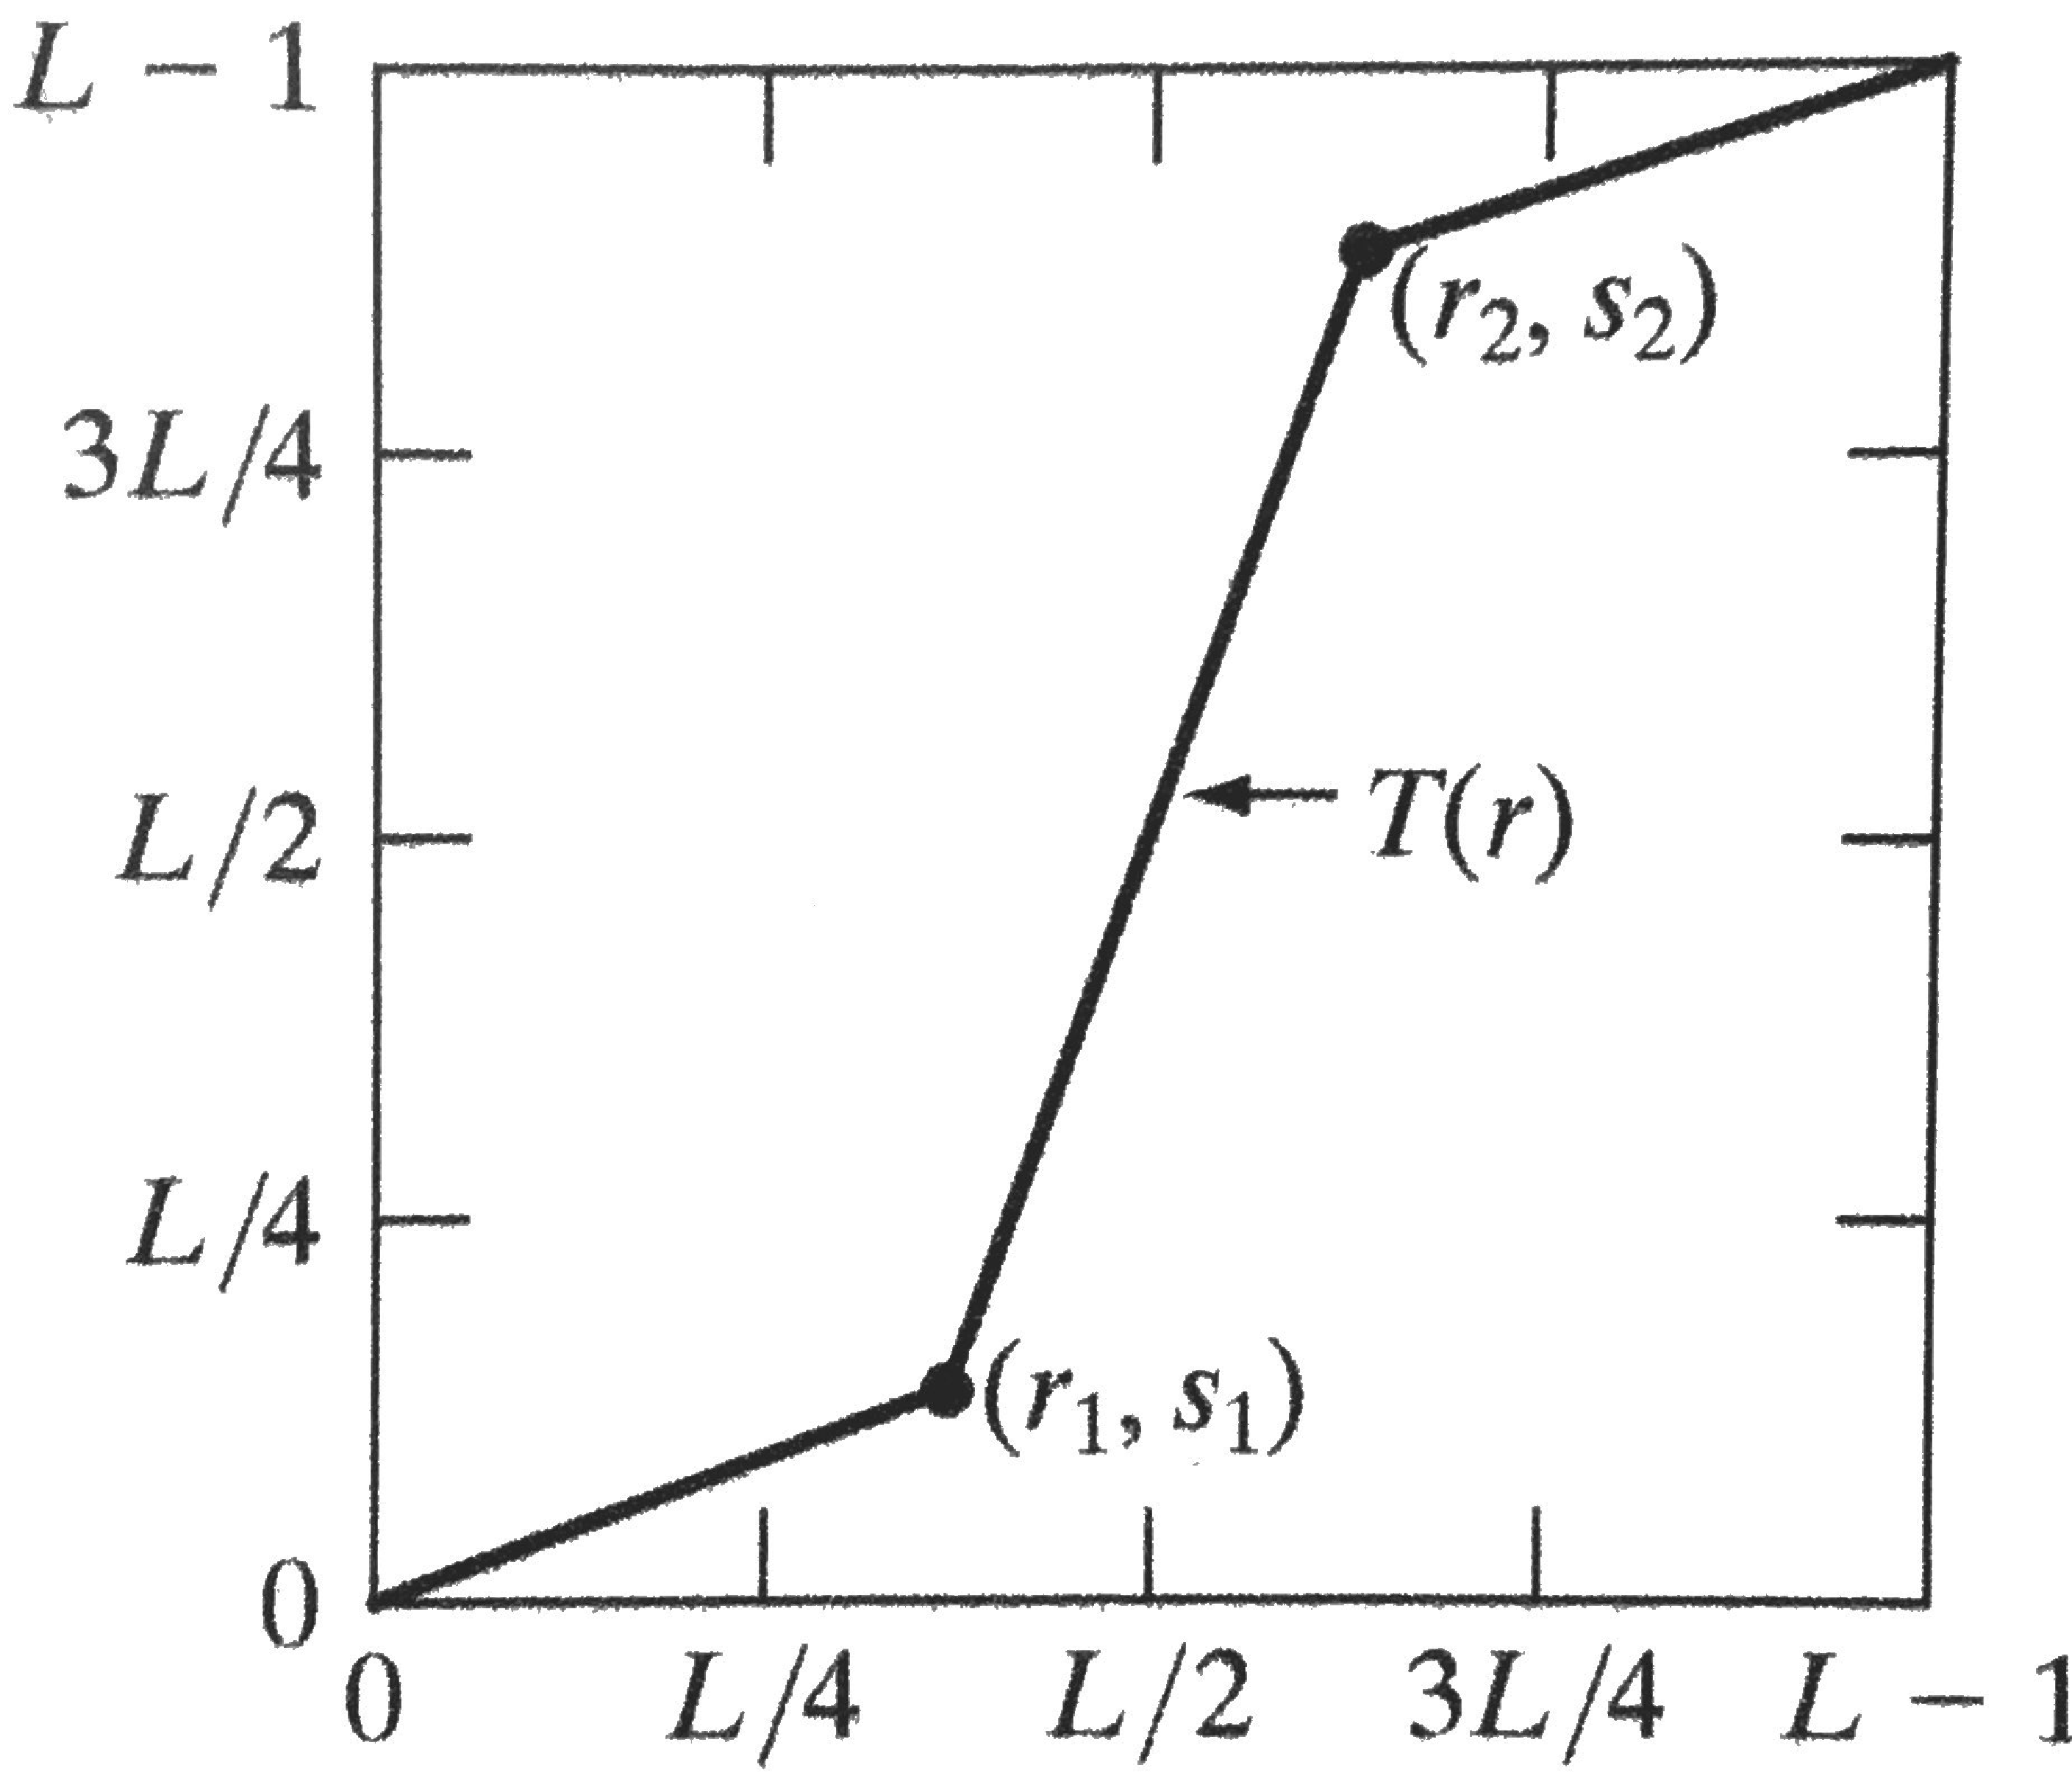
\includegraphics[height=1.55in]{T-Contrast2.pdf}}
\end{picture}%
\par\vspace{.08cm}
\begin{minipage}{5in}
in an image	
is to apply a point operation~$S:\mathbb{P}\rightarrow\mathbb{P}$
that further decreases luminance values that are already low, 
and on the other hand increases large luminance values.
Implement, in \em Matlab \em or \em Python \rm (or any 
programming language that you would rather use)
the a point function~$s=T(r)$ whose graph is given in the figure 
on the right.
Note that the parameters~$(r_1,s_1)$
and $(r_2,s_2)$ 
should be part of the input (i.e.~the arguments) to your function.
\end{minipage}
\end{problem}
\begin{problem}[More on isotropy]
\label{probgrad}
In the last homework you showed that the Laplacian $\nabla^2$
is \em isotropic\em\/.
Isotropy is important if you want an operation to be
rotation-invariant: that is, if you apply the same operation
to an image that has been rotated by a certain angle, you
want it to yield the same result as the operation applied to the non-rotated image. This is important, for example, for edge detection. 
Consider:
\par\vspace{.15cm}
\hfill
$\|\nabla f(x,y)\|=
\sqrt{\big(
	\frac{\partial f}{\partial x}
	\big)^2+
    \big(\frac{\partial f}{\partial y}
\big)^2}$\,,
\hfill
and
\hfill
$\|\nabla f(x,y)\|\simeq
	\big|\frac{\partial f}{\partial x}
	\big|+
	\big|\frac{\partial f}{\partial y}
	\big|$.
\hfill
\mbox{ }
\par\vspace{.15cm}
{\bf(a)}~The first of the above equations is the 
formula for the magnitude of the gradient:
show that it is an isotropic operation.
{\bf(b)}~The second one is an approximation
of~$\|\nabla f\|$: show that this is \em not \em isotropic.
\par
\end{problem}
\begin{problem}[Edge detection]
\label{ed}
{\bf(a)}~The simplest way of detecting 
edges is precisely to compute the magnitude
of the gradient of an image and display it as if it were an image.
Implement code that detects the edge
of \verb|image-contactlens.tif|
(it is a contact lens illuminated by a lighting arrangement
designed to highlight imperfections):
that is, define $J(i,j)=\|\nabla I(i,j)\|$,
where partial derivatives are computed using Sobel filters.
Also, enhance your image with a threshold point function,
i.e.~define $K(i,j)=H(J(i,j)-t)$,
where $H(\cdot)$ is the Heaviside function
($H(x)=1$ for~$x\geq0$, and $H(x)=0$
for $x<0$)
and~$t$ is a treshold selected at~33\% of the 
highest value in the image~$J$. 
{\bf(b)}~Another way to 
detect the edges of an image~$I$ 
is to use the \em Laplacian \em 
of the image~$\nabla^2 I$. Remember that
derivatives of an image (unlike the \em magnitude \em
of its gradient) may 
have \em negative \em values, therefore we should use
either the absolute value~$|\nabla^2 I|$
or the \em positive values \em of the Laplacian,
namely $J(i,j)=\max(\nabla^2I(i,j),0)$.
Why would this work? (Think about the cross section of an edge.)
Implement code that computes and displays the 
positive values of the Laplacian, and apply
it to \verb|image-circuit.tif|
(which shows a \em binary \em portion of a wire-bond
mask for an electronic circuit).
{\bf(c)}~Consider now \verb|image-building.tif|,
which exhibits some pretty regular geometry.
First compute and display~$\|\nabla I\|$;
you will note that all edges, even the minor ones (corresponding to bricks on the walls), are detected
and displayed. 
Edge detection can be made more selective by smoothing the image prior
to computing the gradient.
%If you are only interested in the 
%major edges, it is a good idea to pre-filter the image 
%with a smoothing convolution kernel. 
So, perform the following operations, in this order: (i)~smooth the
original image with a~$5\times5$ mean filter (each entry is equal to 1/25); (ii)~detect the edges by computing the gradient,
using either of the two methods from {\bf Problem~\ref{probgrad}};
and finally (iii)~treshold the resulting image, with the technique described in part~(a), with a threshold equal to 33\% of the highest
value in the image (you may try different  thresholds). Submit your code and your results.
\end{problem}
\par\vspace{.05cm}
\hfill
\begin{minipage}{5.5in}
	{\bf Norms.}
	Let~$V$ be a vector space (think of~$\mathbb{R}^n$).
	Remember that a \em norm \em on~$V$ is a function $\| \cdot \|: V\rightarrow \mathbb{R}$ 
	with the properties:
	{\bf(N1)}~$\|a\mathbf{v}\| = |a|\,\|\mathbf{v}\|$ for all $a\in \mathbb{R}$ and $\mathbf{v}\in V$;
	{\bf(N2)}~$\|\mathbf{v}+\mathbf{w}\| \leq \|\mathbf{v}\|
	+\|\mathbf{w}\|$ for all~$\mathbf{v},
	\mathbf{w}\in V$ ({\it triangle inequality});
	{\bf(N3)}~$\|\mathbf{v}\|=0 \Rightarrow \mathbf{v}
	=\mathbf{0}$ (the zero of~$V$).
	Similarly, a map $\| \cdot \|: V\rightarrow \mathbb{R}$
	with properties~{\bf(N1)} and~{\bf(N2)}, and \em not\em~{\bf(N3)},  is called a
	\em seminorm \em on~$V$.
\end{minipage}
\hfill\mbox{ }
\par\vspace{.05cm}
\begin{problem}[The \em Total Variation \em Norm]
{\bf(a)}~Show, using the 
definition of norm above, that $\|\mathbf{0}\|=0$
and $\|\mathbf{v}\|\geq0$ for all~$\mathbf{v}\in V$ 
(positivity).
{\bf(b)}~We can think of images as elements of a linear 
space (this is technically correct as long as we admit images
with negative values). In fact, let's first consider
\em continuous images\em\/, i.e. defined on the 
continuous domain~$D=[0,M]\times[0,N]$.
A \em measure of sharpness \em of the image
is the so-called \em Total Variation \em (TV) norm: 
\par\vspace{-.35cm}\hfill\mbox{ }\hfill\mbox{ }\hfill\mbox{ }\hfill
$\displaystyle
\label{TVnorm}
\|I\|_\mathrm{TV}=\frac{1}{\mbox{Area}(D)}
\iint_D\|\nabla I(x,y)\|\,dA,
$\hfill\mbox{ }
\par\vspace{.10cm}
which is nothing but the mean value of the magnitude of the gradient
of the image.
Note that the norm in the integral is the usual
Euclidean norm in~$\mathrm{R}^2$: namely
if~$\mathbf{v}=(a,b)$
then $\|\mathbf{v}\|=\sqrt{a^2+b^2}$.
Show that it is, in fact, a \em seminorm \em 
on the set of~$C^1(D)$ functions (functions that are
continuously differentiable in~$D$). Why is it a 
seminorm and not a norm?
{\bf(c)} In the \em discrete \em setting, 
i.e.~for real images~$I:\mathbb{D}\rightarrow\mathbb{P}$,
we compute the TV norm numerically as follows:
\par\vspace{-.35cm}\hfill\mbox{ }\hfill\mbox{ }\hfill\mbox{ }\hfill
$\displaystyle
\|I\|_\mathrm{TV} = 
\frac{1}{M\cdot N}
\sum_{x=0}^{M-1}\sum_{y=0}^{N-1}\|\nabla I(x,y)\|.
$\hfill\mbox{ }
\par\vspace{.1cm}
Write computer code (in \em Python\em\/, or 
 \em Matlab\em\/, or anything else) that computes the Total Variation norm of an
image~$I$, where the partial derivatives in the gradient are computed
using  Sobel filters.
\end{problem}
\begin{problem}(More on sharpening)
{\bf(a)}~In Problem~1.10 of the previous homework assignment we
introduced the so-called Laplace Filter for sharpening:
$J=I-\nabla^2I$. Now consider the modified Laplace Filter
$J=I-k\nabla^2I$, where~$k$ is a positive constant.
Modify the computer program that you wrote last time
to incorporate this constant, and 
apply it to \verb+image-moon.jpg+
for different values of~$k$ 
varying from 0.1 to 4.
For both the original image and 
the outputs compute the~TV norm
using the code from the previous problem. 
{\em Hint:} To avoid \em saturation artifacts \em 
in the image~$J$
(due to negative values or above 255)
you should modify your result~$J$
\mbox{defining~$J_2(i,j)=\min(\max(J(i,j),0),255)$, and use it as
your final result.}
\begin{picture}(0,0)
\put(-105,-175){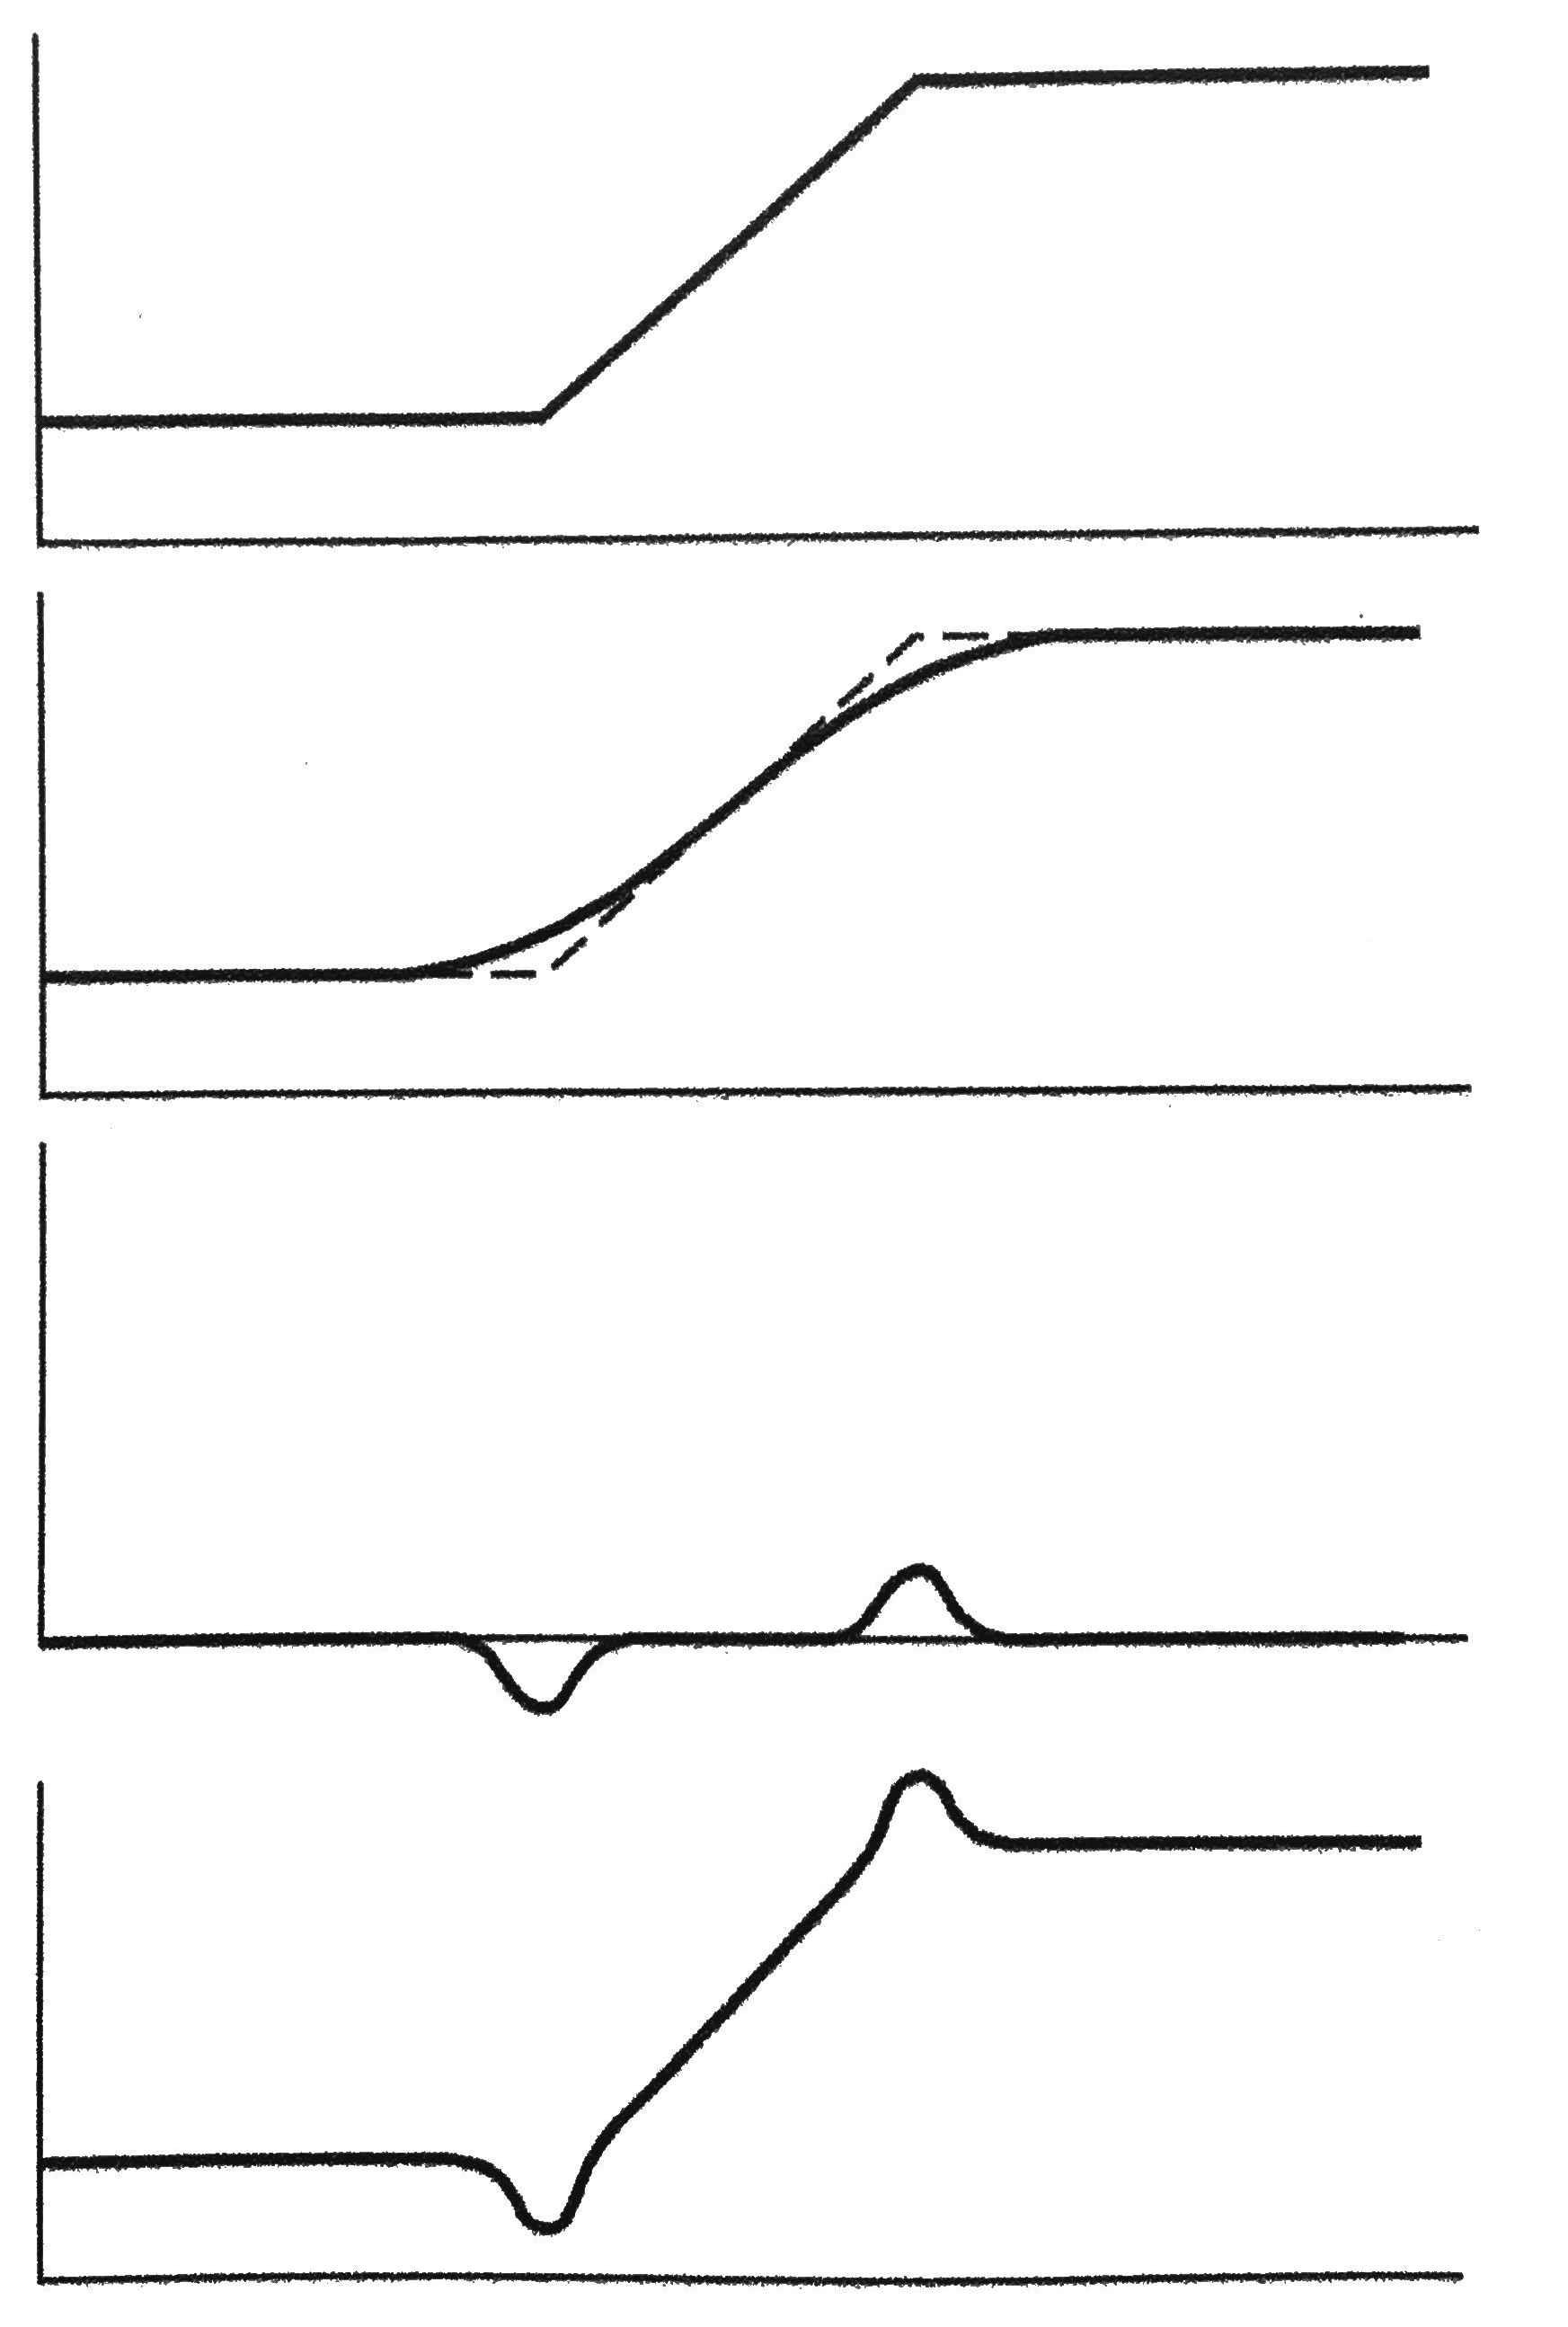
\includegraphics[height=6cm]{USM.png}}
\put(-105,-265){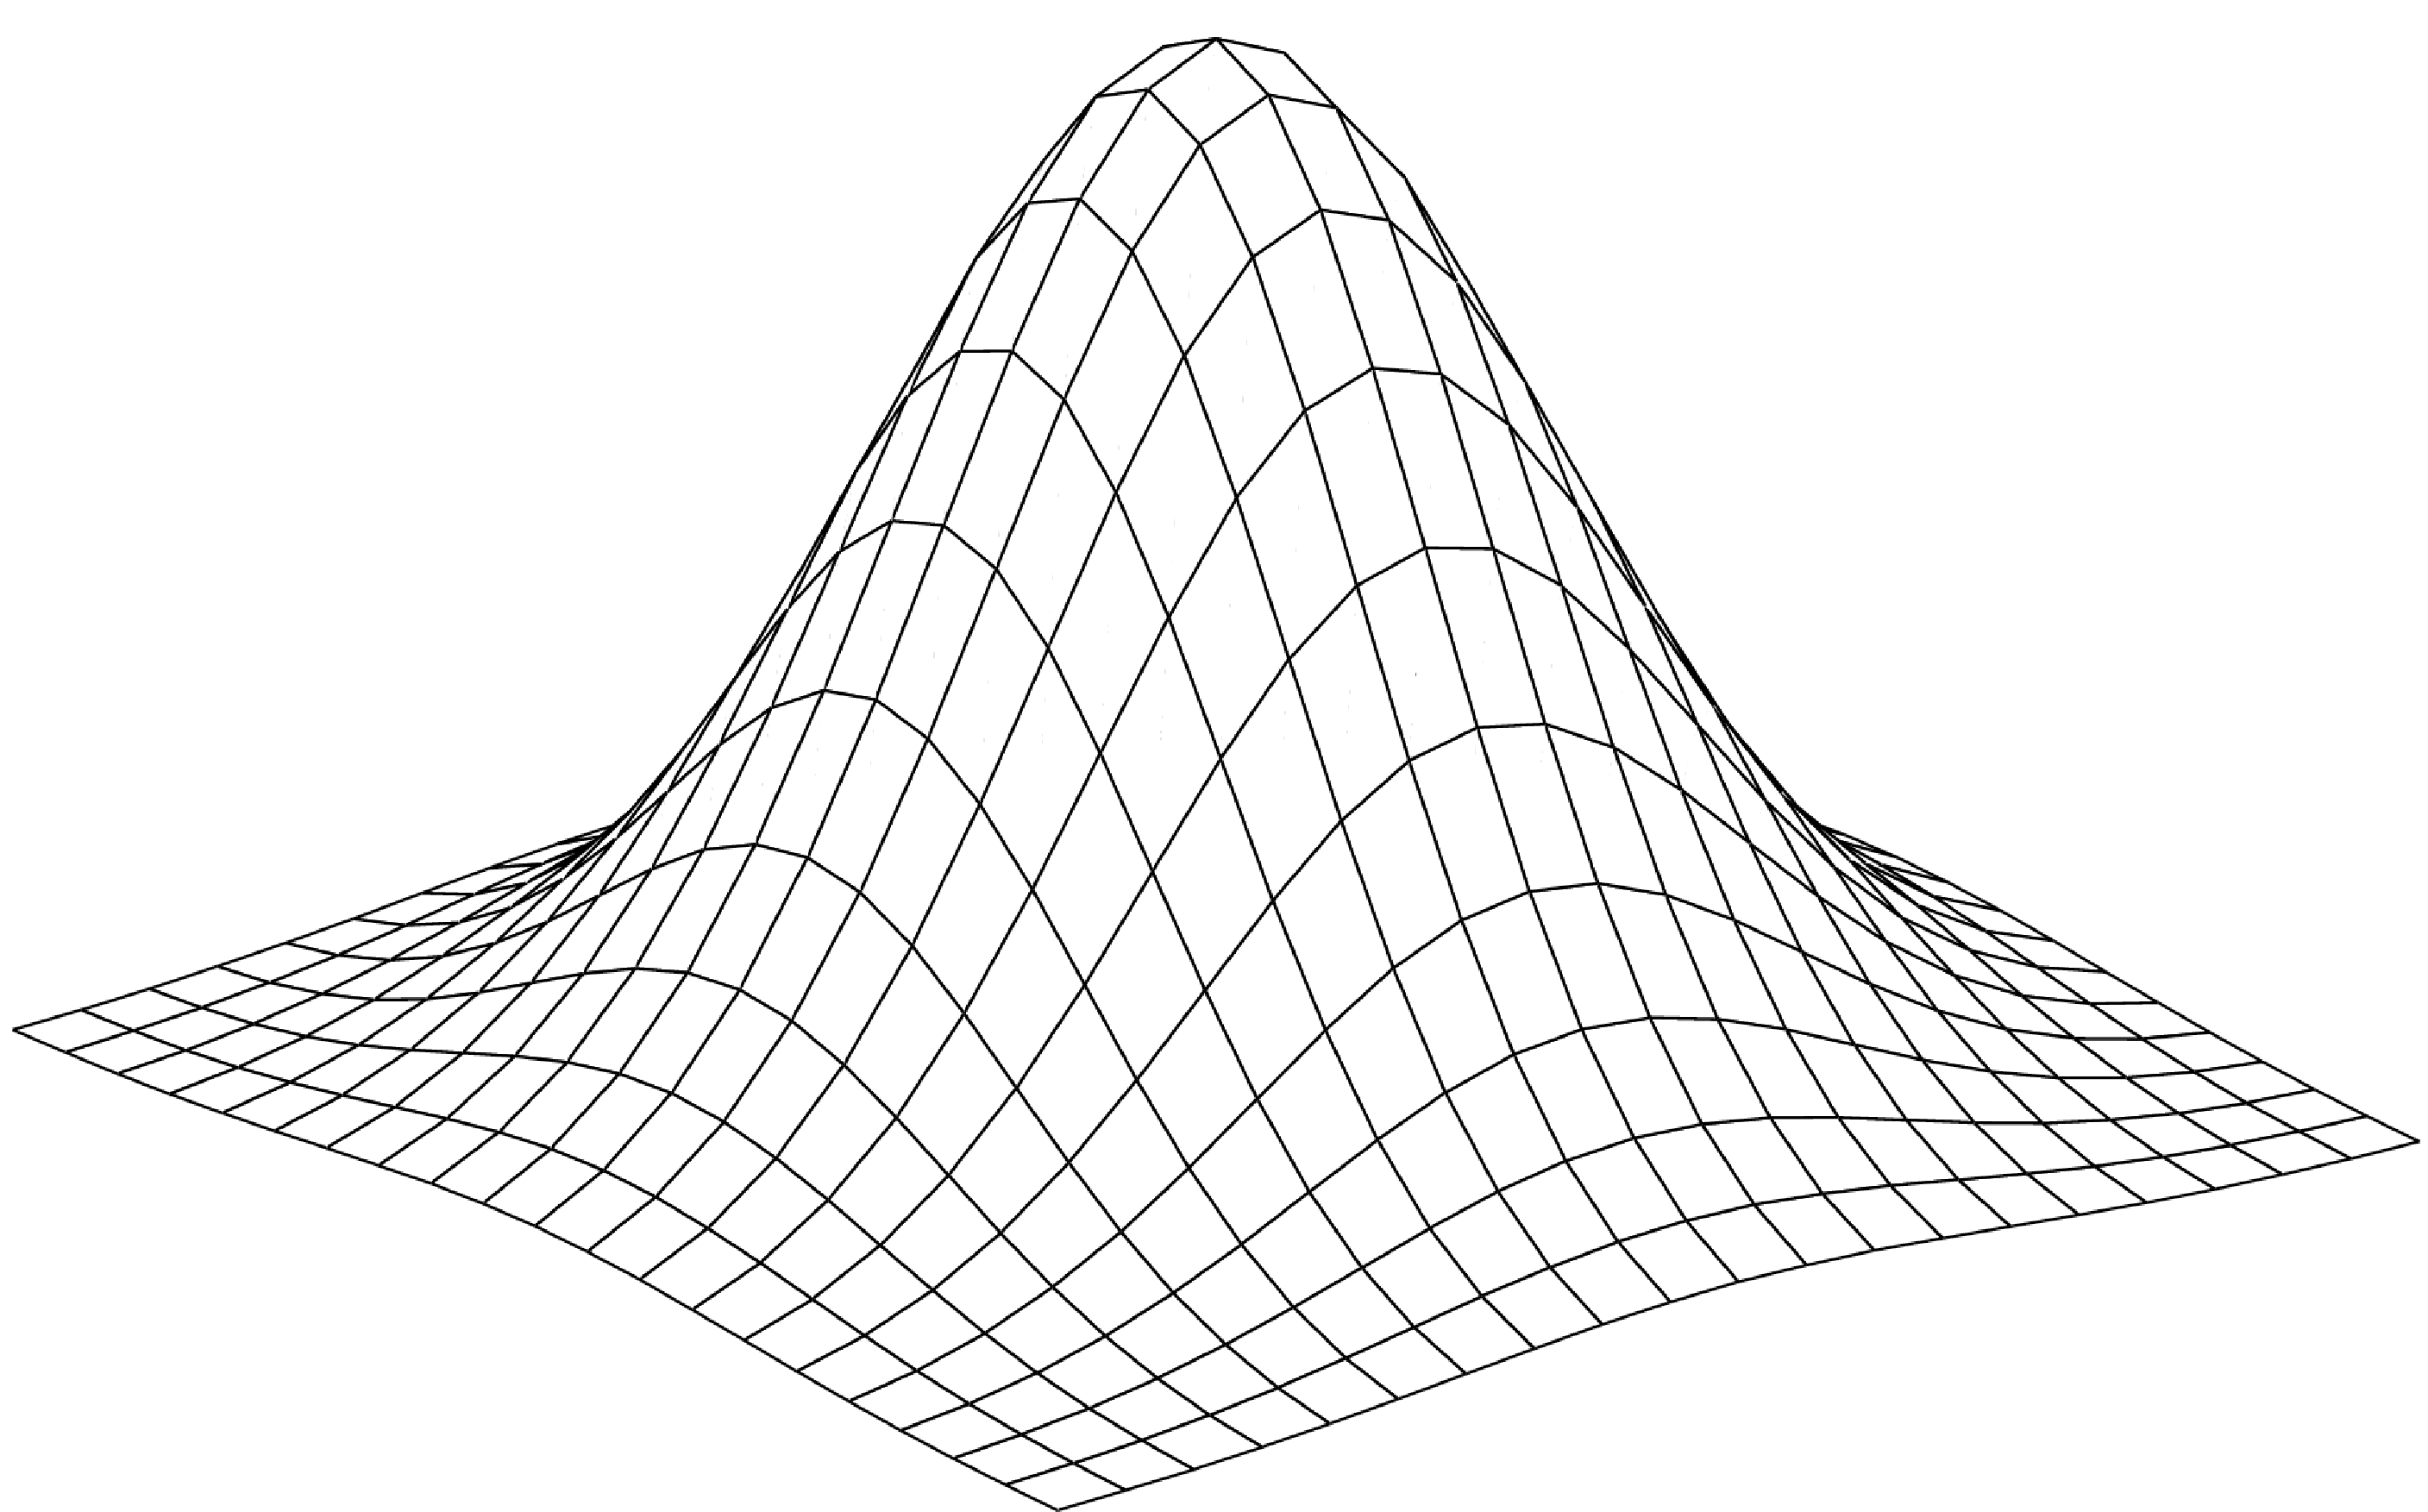
\includegraphics[height=2.5cm]{Bell2.pdf}}
\put(-27.5,-28){\makebox(0,0){$I$}}
\put(-27.5,-70){\makebox(0,0){$M$}}
\put(-27.5,-105){\makebox(0,0){$S$}}
\put(-27.5,-157.5){\makebox(0,0){$J$}}
\end{picture}
\par\vspace{.1cm}
\begin{minipage}{13.25cm}
{\bf(b)}~As we will see in Fourier anaysis, 
the Laplace Filter has the problem that it
may boost the higher frequencies ``too much''.
A way around it is to use the so-called 
\em Unsharp Masking \em (USM), which 
was explained in class. We first compute a
smooth version of the image~$I$,
namely $M=I\ast h_M$, where~$h_M$
is an averaging filter or
a Gaussian mask. We then compute
$S=M-I$, which is the ``sharp
component'' of~$I$ (also known as 
the \em unsharp mask\em\/).
Finally, we add back to~$M$
a ``boosted'' version of the sharp component,
i.e.~$J=M+kS$, with some $k>1$ 
(note that for~$k=1$ we get back the
original image~$I$). We can also write
$k=1+a$, with $a>0$, and write
$J=M+(1+a)S=M+S+aS=I+aS$.
The number~$a>0$ is sometimes called the 
\em sharpening strength\em\/.   
Note that~$a$ is not the only parameter,
as another item that we can choose is the
smoothing convolution kernel~$h_M$:
a common choice is  a $n\times n$ Gaussian mask 
($n$ is odd).
I.e, we fix a standard deviation~$\sigma$
and sample the Gaussian 
bell-shaped function:
\par\vspace{.15cm}
\hfill
$\displaystyle
G(x,y)=\exp\Big(-\frac{x^2+y^2}{2\sigma^2}\Big)$
\hfill\mbox{}\par\vspace{.15cm}
(shown on the right) at integer coordinates, 
and divide the resulting mask by
the sum of its elements (so to obtain 
a mask whose elements sum to one);
$\sigma$ is called the \em spatial extent \em of the filter.
For example,
for~$n=3$ and~$\sigma=2$ we get:
\end{minipage}
\par\vspace{.15cm}
\hfill
$\displaystyle
h_M
=\frac{1}{\sum_{i,j=-1}^1G(i,j)}
\left[
\begin{array}{ccc}
G(-1,-1) & G(-1,0) & G(-1,1)  \\
G(0,-1) & G(0,0) & G(0,1)  \\
G(1,-1) & G(1,0) & G(1,1)  
\end{array}
\right]
=
\left[
\begin{array}{ccc}
0.0449 & 0.1221 & 0.0449  \\
0.1221 & 0.3319 & 0.1221  \\
0.0449 & 0.1221 & 0.0449  
\end{array}
\right].
$
\hfill\mbox{}
\par
\par\vspace{.15cm}
For larger values of~$\sigma$, it is comvenient 
to use a larger convolution kernel size~$n$.
Write code that implements the Unsharp Masking 
method. Ideally your function should 
have, as inputs: $I$ (the image to be sharpened), 
$a$ (the sharpening strength), $\sigma$ (the spatial extent of the Gaussian mask), $n$
(its size); and as output:~$J$
(the sharpened image). Apply it to the image \verb+image-irish.tif+
with~$a=1$ and different values of~$\sigma$, e.g.~$\sigma=2.5$, 
$\sigma=5$, and 
$\sigma=10$. 
For both \verb+image-irish.tif+ and each resulting
image, also compute the TV norm.
Please turn in both your code and your results.
\par\vspace{.15cm}
{\em Remark:} 
Here is some food for thought. Different regions of
an image may need different sharpening strenghts---which leads to
the idea of \em adaptive sharpening\em. That is, 
one can define: $J(i,j)=I(i,j)+a(i,j)S(i,j)$,
where the sharpening strength~$a$ depends on the location~$(i,j)$.
The simplest way to implement this is to set
$a(i,j)=H(\|\nabla I(i,j)\|-t)$, where~$H$ is 
the Heaviside function ($H(x)=1$ for~$x\geq0$, and $H(x)=0$
for $x<0$) and~$t$ is a user-defined threshold:
that is, we have $J=I+S$ where $\|\nabla I\|$ 
is larger than~$t$, otherwise it is left unchanged~($J=I$).
Can you think of other ways to implement adaptive sharpening?
(You don't have to answer this question,
but it may be material for a future project.) 
\end{problem}
\begin{problem}[Detecting diagonal edges]
The techniques that we have seen 
so far can be used to detect%
\begin{picture}(0,0)
\put(-120,-50){$h_{\mathbf{n}}
	=
	\frac{1}{8}
	\left[
	\begin{array}{crr}
	2 & 1 & 0 \\
	1 & 0 & -1 \\
	0 & -1 & -2
	\end{array}
	\right]$}
\end{picture}
\par\vspace{.05cm}
\begin{minipage}{12.5cm}
	edges that are parallel to a prescribed direction. 
	For example, 
	if~$\mathbf{n}=(a,b)$
	is a unit vector (that is,~$\sqrt{a^2+b^2}=1$) that
	is \em orthogonal \em to a particular direction that
	we are interested in, we can find
	the points $(x,y)$ where the \em directional derivative \em
	of~$I$ in the direction~$\mathbf{n}$, defined as
	the number
	\par\vspace{.15cm}
	\hfill
	$
	\displaystyle
	\frac{\partial I}{\partial \mathbf{n}}
	(x,y)
	=\lim_{h\rightarrow0}
	\frac{I(x+ah,y+bh)-I(x,y)}{h},
	$
	\hfill\mbox{ }
	\par\vspace{.15cm} 
\end{minipage}
\par
is large (in absolute value). The above formula (which should be familiar from multivariable calculus) is valid in a continous setting;
for digital images it is approximated with discrete 
filters, as it is the case
for the partial derivatives $\partial I/\partial x$ and
$\partial I/\partial y$. For example, for~$\mathbf{n}=(1,1)/\sqrt{2}$
(remember that we always consider~$x$ pointing downwards and~$y$
poiting right!)~the corresponding Sobel filter~$h_{\mathbf{n}}$ is shown above.
Consider again \verb|image-building.tif|, 
used in {\bf Problem~\ref{ed}}.
Smooth it with a~$5\times5$ mean filter, filter it with the
convolution kernel~$h_{\mathbf{n}}$, compute the absolute
value of the result and display it (you may also to 
treshold the resulting image  with a threshold equal to 33\% of its highest
value). What is highlighted?
\end{problem}
\begin{problem}
Suppose that~$g$ and~$h$ are two convolution kernels,
of sizes $(2K_1+1)\times(2K_1+1)$ and 
$(2K_2+1)\times(2K_2+1)$. What is the size
of the convolution kernel $f=g\ast h$?
Justify your answer.
\end{problem}
\begin{problem}[Image Equalization]
We introduced a technique for \em equalizing \em
an image. Namely,
we defined the \em histogram \em 
and the cumulative distribution function
(CDF) of an image as follows:
\par\vspace{.1cm}
\hfill
$h_I(\ell)=\#\big\{
(i,j)\big|I(i,j)=\ell
\big\},$
\hfill
and\hfill
$\displaystyle
F_I(\ell)
=\frac{L-1}{MN}\sum_{k=0}^{\ell}h_I(k)$,
\hfill
both defined for~$\ell\in\mathbb{P}$.
\hfill\mbox{ }
\par\vspace{.1cm}
We showed that, in the discrete setting, %(in which we are)
defining %the new image
$J(i,j)=F_I(I(i,j))$, $(i,j)\in D$,
yields a new emage whose histogram is 
\em equalized\em\/, in the sense
that while it is not quite true that $h_J$
is a constant, is is tha case that
$F_J(\ell)\simeq\ell$, for $\ell\in\mathbb{P}$.
(In the continuous setting, however, we would obtain a constant 
density for~$J$.)
\begin{enumerate}[\hspace{.25cm}\bf(a)]
	\item Would a second pass of histogram equalization produce a different result?
	\item Write code to implement the above histogram equalization technique (ideally, write a function that has an image as an input
	and the equalized image as an output). 
	Please turn in the code.
	\item Download the image \verb+image-spine.tif+,
	and print it.
	Compute and print its histogram as well as the graph 
	of its cumulative distribution function
	(CDF, as a continuous curve). 
	Now perform histogram equalization.
	Display the new image, compute and display 
	its histogram, as well as the graph 
	of its cumulative distribution function.
	The hard work is done, 
	so repeat part~(c) for \verb+image-fruits.tif+.
	
\end{enumerate}
\end{problem}
\end{document}












